\section{Method}

\subsection{Data preprocessing and feature construction}

The data pipeline starts from one month of ADRR-derived trajectories. Following repository preprocessing, raw tracks are segmented into missions using time-gap rules, resampled to a 5-minute grid, and enriched with both numeric motion features and mask features. The final model consumes 18 numeric features, 2 mask features (\texttt{observed\_flag} and \texttt{gap\_flag}), 9 context features, input H3 region tokens, and parent H3 region tokens.

The use of explicit mask channels is important even though the current paper does not yet introduce a dedicated uncertainty-aware missing-data model. It preserves information about which sequence steps are directly observed and which arise from gap handling.

\subsection{Hierarchical H3 forecasting baseline}

The baseline model is a hierarchical GRU forecaster. The input sequence is embedded through region embeddings, parent-region embeddings, numeric projections, and mask projections. A GRU encoder produces a sequence summary, which is fused with context features. For each horizon, the model predicts coarse parent-region logits, airborne/landed status logits, and child logits conditioned on the predicted coarse region.

This design already offers a strong and scalable spatial prior, but it compresses all horizons into one shared temporal summary. We found this to be the main temporal bottleneck.

\subsection{Horizon-query Transformer decoder}

To address that bottleneck, we replace the recurrent sequence summarizer with a horizon-aware query decoder. The single-scale Transformer variant works as follows: (1) project concatenated sequence features into a Transformer hidden dimension, (2) add learned positional embeddings and run masked self-attention over the history, (3) compute a masked mean summary of encoder states and fuse it with context features, (4) introduce one learned horizon embedding and one learned query per forecast horizon, (5) use each horizon query to attend over the encoded history sequence, and (6) fuse the shared summary, the horizon-attended representation, and the horizon embedding into a horizon-specific decoder feature. This decoder feature is then fed into the same hierarchical H3 output heads.

\subsection{Proposed multiscale horizon-query Transformer}

Our final model adds an explicit second temporal scale on top of the Transformer horizon decoder. The proposed architecture contains two temporal branches: a fine-scale Transformer encoder over the original resampled sequence, and a coarse-scale Transformer encoder over a stride-pooled version of that sequence.

\begin{figure}[!t]
\centering
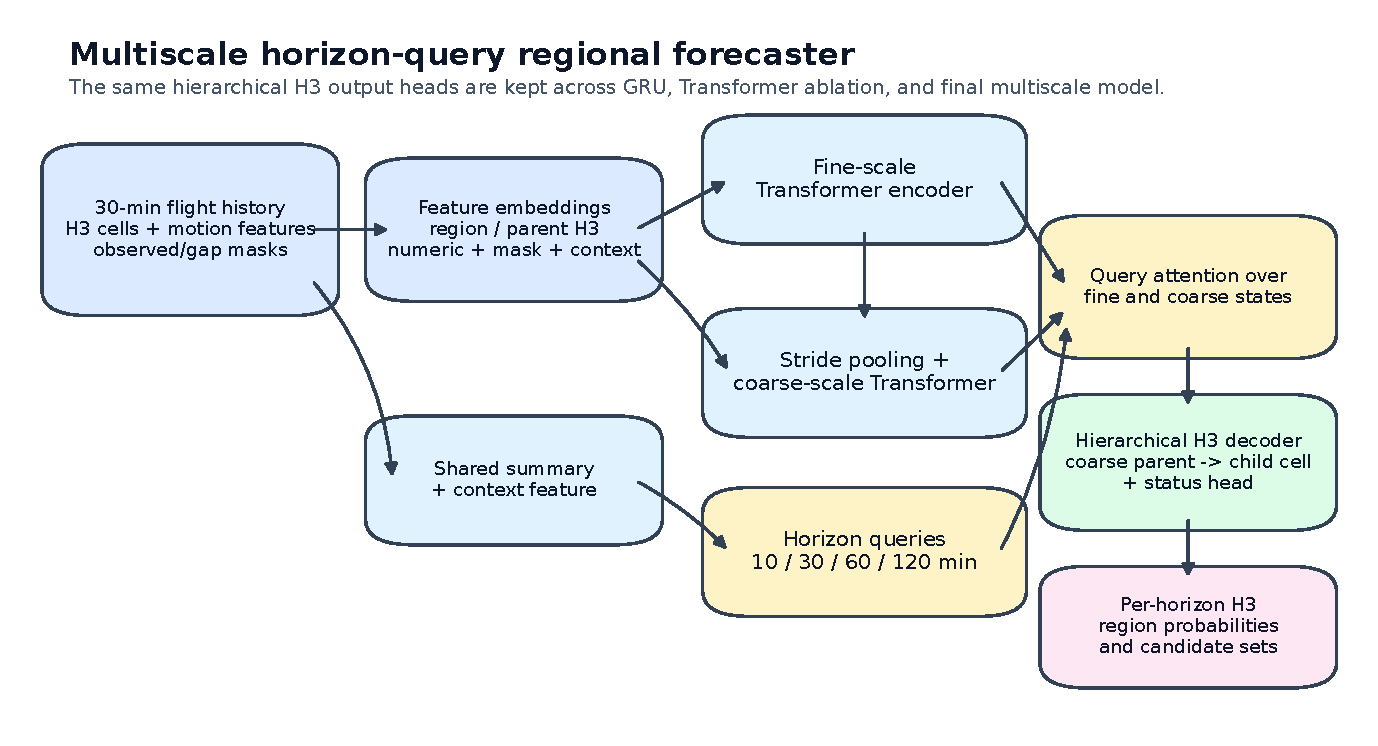
\includegraphics[width=\textwidth]{figures/fig1_method_architecture.pdf}
\caption{Overview of the proposed multiscale horizon-query H3 forecaster. The same hierarchical output heads are used across all model variants, but the final model augments the single-scale horizon-query decoder with an explicit coarse temporal branch.}
\label{fig:method-architecture}
\end{figure}

For each horizon query $q_h$, we compute attention over both the fine sequence and the coarse sequence,
\begin{equation}
\alpha_h^{(f)} = \mathrm{softmax}(q_h K_f^\top), \qquad
\alpha_h^{(c)} = \mathrm{softmax}(q_h K_c^\top),
\end{equation}
and obtain attended representations
\begin{equation}
z_h^{(f)} = \alpha_h^{(f)} V_f, \qquad
z_h^{(c)} = \alpha_h^{(c)} V_c.
\end{equation}
These are fused with the shared context feature and the horizon embedding,
\begin{equation}
d_h = \phi([b; z_h^{(f)}; z_h^{(c)}; e_h]),
\end{equation}
where $b$ is the shared base feature, $e_h$ is the horizon embedding, and $\phi(\cdot)$ is a small projection block. The resulting $d_h$ is then used for coarse-region prediction, status prediction, and coarse-conditioned child prediction.

This multiscale design preserves the main advantage of the single-scale horizon-query decoder while improving access to longer-term temporal structure.

\subsection{Training objective}

The main loss is the average of cross-entropy over coarse H3 classes, cross-entropy over valid child classes, and cross-entropy over airborne/landed status. We also implemented an optional adjacent-horizon consistency penalty over decoder features, but in our experiments its contribution was not beneficial enough to retain in the final model. Therefore, the final submitted variant uses the tuned multiscale architecture without consistency regularization.

\subsection{Optional H3-neighbor refinement}

We further evaluate an inference-time spatial postprocessor that diffuses a fraction of fine-cell probability mass to local H3 neighbors. This is not part of the final model. Its purpose is to test whether lightweight spatial smoothing can improve candidate-region recall. As shown later, it increases candidate coverage but noticeably harms calibration, so we keep it as an ablation.
